Let $A$ denote the area, and $h$ the height of the triangle. 
\begin{figure}[H]
\centering
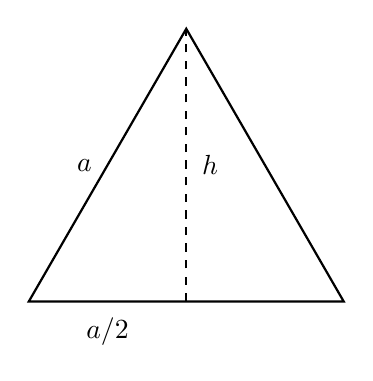
\begin{tikzpicture}[thick, sharp corners, inner sep=1mm, outer sep =1mm, scale=4]
\draw (0,0) -- (0.5,0) node[midway,below]{$a/2$} -- (1,0) -- (0.5, 0.866) -- cycle node[midway,left]{$a$}; 
\draw[dashed] (0.5,0) -- (0.5,0.866) node[midway,right]{$h$};
\end{tikzpicture}
\end{figure}
The area of the triangle is given by one-half the product of the base and height:
\begin{align*}
A = \frac{1}{2} ah
\end{align*}
The height $h$ is unknown, but can be found by an application of the Pythagoras theorem.
\begin{align*}
& h^2 + \left(\frac{a}{2}\right)^2 = a^2 \\
\Rightarrow
h^2 & = a^2 - \frac{a^2}{4} 
      = \frac{3a^2}{4}
\end{align*}
And thus,
\begin{empheq}[box={\mathbox[colback=white]}]{equation*}
    h = \frac{a}{2} \sqrt{3}
\end{empheq}
\begin{empheq}[box={\mathbox[colback=white]}]{equation*}
    A = \left(\frac{a}{2}\right)^2 \sqrt{3}
\end{empheq}
